%&latex2e

\documentclass[twoside,draft]{article}
\usepackage{latexsym,conference}

\usepackage[letterpaper]{geometry}
\usepackage[utf8]{inputenc}
\usepackage[english]{babel}

\usepackage{amssymb,amsfonts,amsmath}

\usepackage[perpage,symbol*]{footmisc}
\usepackage[final]{graphicx}
\usepackage{pstricks}
\usepackage{cite}

\usepackage[varg]{txfonts}

\oddsidemargin=-0.20in
\evensidemargin=-0.20in
\topmargin=-30pt

\textwidth=498pt
\textheight=646pt


\begin{document}
%\begin{tableofcontents}
\begin{sloppypar}

\renewcommand{\refname}{References}
\renewcommand{\tablename}{\small Table}
\renewcommand{\figurename}{\small Fig.}
\renewcommand{\contentsname}{Contents}


\twocolumn[%
\begin{center}
\renewcommand{\baselinestretch}{0.93}
{\Large\bfseries HOLOEXPO CONFERENCE IN HOLOGRAPHY

}\par
\renewcommand{\baselinestretch}{1.0}
\bigskip
F. M. Sanchez$^1\!$, \ V. A. Kotov$^2\!$, \ M. Grosmann$^3$, \ D. Weigel$^4$, \ R. Veysseyre$^5$,\\ \ C. Bizouard$^6$, \ N. Flawisky$^7$, \ D. Gayral$^8$, \ L. Gueroult$^9$\\
{\footnotesize  $^1$ Pr. Universit\'{e} Paris 11, Orsay, France (retired).\rule{0pt}{12pt}
E-mail: hol137@yahoo.fr\\
$^3$ Pr. at Universit\'{e} Louis Pasteur, Strasbourg, France (retired). michelgrosmann@me.com
$^7$Architect / Math Instructor at ENSA Ecole Nationale Sup\'{e}rieure d'Architecture, Paris Malaquais, France. flawisky@free.fr
$^9$Lecturer at ENSA Paris Malaquais, France (retired). lgueroult@hotmail.com

}\par
\medskip
{\small\parbox{11cm}{%
\hfill To the memory of Sir Michael Atiyah\\
The antique concept of permanent Cosmos is reintroduced as a perfect deterministic computer, inverting the anthropic principle and interpreting the dimensionless parameters as optimal calculation bases. The later are unified in the Topological Axis, which exhibits the string theory dimension series 4k+2, with the emphasis on the values 26 (visible Universe) and 10 (the Hydrogen - Pion couple). The 1D extension of the Holographic Principle defines the Grandcosmos and a $10^{61}$ trans-Plankian quantified time. This confirms the matter-antimatter Oscillatory Bounce and resolves at last the vacuum energy dilemma. The mathematics-physics fusion is proved by $10^{-9}$ precise relations, showing Four Force Unification with the Eddington's constant 137 and the Atiyah's one. The Holic Principle and Eddington's Theory must unlock Particle Physics, with massive gluons and composite d quark. Based on the imperfect cosmological principle, the standard evolutionary cosmology will be excluded by the observation of mature galaxies in the very far-field, and also by the invariance of the CMB temperature.  

%Mature galaxies will be found in the far-field instead of a dark space, rejecting thus the evolutionary cosmology, ill-founded %o%%n the imperfect cosmological principle.

%% TODO: Insérer axe topologique
}}\smallskip
\end{center}]{%


\setcounter{section}{0}
\setcounter{equation}{0}
\setcounter{figure}{0}
\setcounter{table}{0}
\setcounter{page}{1}


\markboth{F.M. Sanchez,\ M. Grosmann,\ B. Kress,\ N. Flawisky,\ L. Gueroult, \textit{Cosmic Holography}}{\thepage}
\markright{F.M. Sanchez,\ V.A. Kotov,\ M. Grosmann,\ D. Weigel,\ R. Veysseyre,\ C. Bizouard,\ N. Flawisky,\ D. Gayral,\ L. Gueroult, \textit{Back to Cosmos}}
Contents
\markright{F.M. Sanchez,\ M. Grosmann,\ B. Kress,\ N. Flawisky,\ L. Gueroult, \textit{Cosmic Holography}}

1. The Principles of Hierarchy and Computation

2. Special holographic relations

~~~    7.1. The conservation of information
   
~~~    7.2. The cosmic temperature

~~     7.3. The Holic Principle and CCO 
    
   
 3. Discussion
 
 4. Conclusions
 
    
\markright{F.M. Sanchez,\ M. Grosmann,\ B. Kress,\ N. Flawisky,\ L. Gueroult, \textit{Cosmic Holography}}
\section{The Principles of Hierarchy and Computation}
\markright{F.M. Sanchez,\ M. Grosmann,\ B. Kress,\ N. Flawisky,\ L. Gueroult, \textit{Cosmic Holography}}

It was observed that the physical constants are tightly contrived, but only three dimensionless parameters: $a$, $p$, and $a_{G}$ are sufficient to explain the main structures of the world \cite{Carr}. Two of them are precisely measured: the electric constant $a$ $\approx$ 137.035999139(31), known with 0.23 ppb precision, and the proton-electron mass ratio $p$ $\approx$ 1836.15267245(75), known with 0.41 ppb precision. The gravitational coupling constant $a_{G}$ was the square of the ratio Planck/proton mass, subjected to a relatively large imprecision 10$^{-4}\!$ due to the imprecision on $G$ measurement. In fact, the authors condidered rather the inverse of $a$ and $a_G$, noted $\alpha$and $\alpha_G$. The present article will show that our notation, following Eddington, is far more appropriate.

One can read \cite{Carr}: \textit{“For example, the size of a planet is the geometric mean of the size of the Universe and the size of an atom; the mass of man is the geometric mean of the mass of a planet and the mass of a proton. Such relationships, as well as the basic dependencies on $\alpha$ and $\alpha_G$ from which they derive, might be regarded as coincidences if one does not appreciate that they can be deduced from known physical theory, with the exception of the Universe, which cannot be explained directly from known physics... This line of arguments, which is discussed later, appeals to the 'anthropic principle'.”}

The existence of relations that are not explained by known physical theories, is called 'natural fine tuning' phenomena. But, as soon as it involves the observable Universe radius, it signals the existence of a fundamental theory that must take into account the \textit{antique Cosmos concept, which, as Eddington claimed \cite{Eddington}, must be permanent}. Extending this to the standard spatial homogeneity, this leads to the Perfect Cosmological Principle, the very foundation of the steady-state cosmology and the starting point of Coherent Cosmology \cite{Sanchez1}.

Eddington interpreted rightly the Cosmic Large Number correlations, as recalled in this article. However, his work was rejected for obscure reasons and this rejection was enforced by the fact that about 30 dimensionless parameters appear as 'free parameters' in the Particle standard model. They are misnamed since far from being really 'free', they are imposed by Nature. Nevertheless, a large majority of theorists believe they are due to chance, leading to a separation between Physics and Mathematics, not to speak of Biology. Thus, through the above Anthropic Principle, a majority believe in the Multiverse conundrum, a multiplicity of sterile Universe \cite{Carr}.

\textit{This article shows that physics is a unique part of presently incomplete mathematics}. We refute here the Multiverse hypothesis by showing very precise fine-tuning (untill $10^{-9})$ between main physical and the mathematical constants: $\pi$, $e$ and $\gamma$, the Euler-Mascheroni constant. Also, this study implies the 26 sporadic groups and confirms the super-string theory, but with complete rehabilitation of the \textit{tachyonic} bosonic string theory.

\textit{A decisive point of physics is the energy conservation, the First Principle of Thermodynamics.} Theorists associate it with time uniformity, but a more direct and logical explanation is that cosmos is a computer, so Intelligent Life receives a justification: to help the cosmological computation. This Inverted Anthropic Principle answers the first of all questions: why one asks questions? We propose that the parameters are optimal bases in a deterministic computing Cosmos. They appear indeed in DNA characteristics and triple-point temperatures of mammals and main molecules \cite{Sanchez1}.

\textit{This reinstates the Laplace determinism}, involving non-local hidden variables, which are identified with the Cosmos, so rejecting the standard Copenhagen statistical interpretation of quantum mechanics.

The fact that three parameters, among 30, are so clearly emerging means that physics, and more generally science, follows a Hierarchical Principle: \textit{one can progress without knowing the details of the underlying fundamental theory.}

So, when Proust and Dalton found whole numbers in chemical reactions, they were prefiguring atomic physics. The same for Balmer, spectral lines and wave mechanics. Idem for Mandeleiev, atomic masses and nuclear physics. Also, when Mandel found whole numbers in biology, he anticipated genetics. 

In the same manner, \textit{this article prefigures the fundamental theory, but precising its arithmetical foundation: the Holic Principle}, recalled in section 6. Thus, there must exist multi-base algorithms able to explain the compatibility between these two principles, Hierarchy and Computation, which seems at first sight somewhat contradictory. 

\markright{F.M. Sanchez,\ V.A. Kotov,\ M. Grosmann,\ D. Weigel,\ R. Veysseyre,\ C. Bizouard,\ N. Flawisky,\ D. Gayral,\ L. Gueroult, \textit{Back to Cosmos}}

\begin{figure*}
\centering
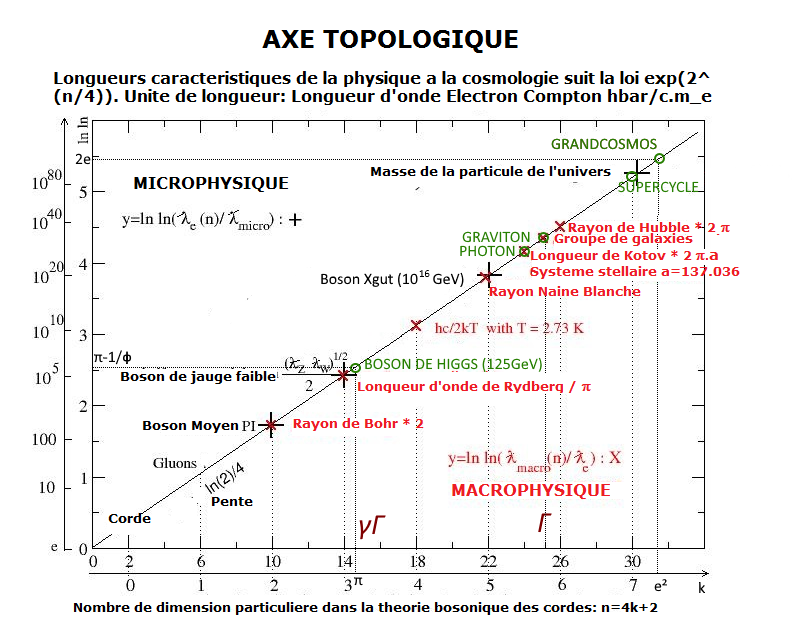
\includegraphics[width=\textwidth,height=14cm]{./figures/figure}
\caption{\textit{The Topological Axis}. The double natural logarithms (y = lnln(Y)) of the main dimensionless physical quantities (Y) corresponds to the special string dimension series n = 4k + 2, from k = 0 to k = 7, showing the Bott
periodicity $\delta n = 8$ [19]. This is the origin of the name `Topological Axis`. 
\textit{In the macro-physics side, with length unit the Electron Compton reduced wavelength} the Universe circumference 
    is tied to the bosonic critical dimension 26, while Bott reduction $\delta n = 8$ leads to n = 18: thermal photon (Cosmological Microwave Background), tied to the the mammal wavelength through the Sternheimer scale factor j (section 8.2); n = 10 (super-string dimension): Hydrogen atom, and n = 2: string. For the number 24 of transverse dimensions, it is
    the Kotov length (section 4.3), through a factor 2$\pi a$, with $a \approx 137.036$. For $n \approx \Gamma $, the Atiyah constant (section 8.2), it is the galaxy group radius, a characteristic cosmic length ($10^{6}$ ligth-years, section 2.1). For $k \approx e^{2}$, $y \approx 2e$, it is the Grandcosmos radius (section 3). The Space-Time-Matter Holic dimension n = 30 (section 6) is tied to $c$ times the cosmic Supercycle period (section 5). \textit{In the micro-physics side, with the same length unit, the Electron Compton reduced wavelength}, Bott reductions from n = 30 lead to the gauge bosons: n = 22 for the GUT bosons, ($10^{16}$ GeV), n = 14 for the weak bosons and for n = 6 for the (\textit{massive}) gluons, about 10 MeV.
    For the intermediary superstring value n = 10, there are the Pions. For $k \approx \pi$, n $\approx \gamma \times \Gamma$, Y $\approx 496^2$ 
    the square of the Green-Schwarz string dimension and the tenth root of the Monster cardinal, it is
    the Brout-Englert-Higgs boson (125 GeV). For k $\approx 2e^e$, it is the topon, the visible Universe wavelength,
    which identifies with the mono-radial unit length of the Bekenstein-Hawking Universe entropy (section 3).
   \textit{With unit the electron mass}, n = 24 would correspond to the photon mass, while n $\approx \Gamma$, 
    to the graviton mass \cite{sanchez1}.
    \textit{With unit the Kotov length}, the holic dimension n = 30 corresponds to the Monster group cardinal order, 
    apart a $\sqrt2$ factor.}
    \textit{The central dimension is n = 16, suggesting that the whole schema is tied to the Eddington's matrix $16 \times 16$}.
\label{fig:figure_label}
\end{figure*}


\markright{F.M. Sanchez,\ M. Grosmann,\ B. Kress,\ N. Flawisky,\ L. Gueroult, \textit{Cosmic Holography}}
\section {The Cosmic Fine-Tuning and the Topological Axis}
\markright{F.M. Sanchez,\ V.A. Kotov,\ M. Grosmann,\ D. Weigel,\ R. Veysseyre,\ C. Bizouard,\ N. Flawisky,\ D. Gayral,\ L. Gueroult, \textit{Back to Cosmos}}

We look here for a systematic organization of dimensionless physical quantities stemming from cosmology, astrophysics, particle   physics, theoretical physics and mathematics. The most famous fine tuning implies cosmic quantities, awkwardly called the `Double Large Number Problem`. If it is a `problem` for standard evolutionary cosmology, it is a precious clue in the steady-state cosmology based on the \textit{Perfect} Cosmological Principle (spatial \textit{and} temporal homogeneity).
This Cosmological Fine-Tuning leads directly to a \textit{Gravitational Hydrogen molecule model of the visible universe} \cite{Sanchez1}.
This defines the Universe horizon radius $R = 2a_{G} \lambdabar_{e}$, where the factor 2 comes from the bi-atomic structure, and where $\lambdabar_{e} = \hbar/cm_{e}$ is the Electron Compton reduced wavelength, while the gravitational coupling constant is: $a_{G} = \hbar c/Gm_{p}m_{H}$, where $m_p$ and $m_H$ are the proton and hydrogen atom masses. So, \textit{the speed $c$ is eliminated}, in accordance with Coherent Cosmology which needs signal celerity far exceeding $c$. This gives $R \approx 13,812~Gly $, corresponding to a Hubble constant 70.790 (km/s)/Megaparsec, compatible with the most recent measurements \cite{Bonvin}: 72(3) (km/s)/Megaparsec. The latter confirms the value measured by the 1a type novae, while the standard optimization of 6 parameters results in a lower value, by $9\%$.

Consider the wavelength of the visible Universe with critical mass $M= Rc^2/2G$: $$\lambdabar_{M} = \hbar /Mc \approx 4.00 \cdot 10^{-96} m$$. This `topon` corresponds to the value $n \approx 2e^e$, close to the touchstone n = 30 of the Topological Axis, see Fig. 1. This scheme illustrates the function $f(n + 4) = f^{2}(n)$
and stems from the imbrication of relations of the form $\lambdabar_{e} /l_{micro} \sim (l_{macro} /\lambdabar_{e})^{2}$, followed by $ l_{macro} /\lambdabar_{e} \sim (\lambdabar_{e} /l^{\prime}_{micro} )^{2}$, leading to:
$$
\begin{array}{ll}
%
\displaystyle
\lambdabar_{e}/\lambdabar_{M} \sim (R/\lambdabar_{e})^{2} \sim (\lambdabar_{e}/ \lambdabar_{X})^{4}\\[+8pt]  % 1st row
\sim (\lambda_{CMB}/ \lambdabar_{e})^{8} \sim (\lambdabar_{e}/\lambdabar_{W})^{16} \sim (2r_{H} /\lambdabar_{e})^{32}\\[+8pt] % 2nd row
\sim (\lambdabar_{e}/ l_{Gl} )^{64} \sim (\lambdabar_{str} /\lambdabar_{e} )^{128} \sim 2^{256}\\ % 3rd row
\end{array}
$$
This series include the Cosmic Microwave Background wavelength $\lambda_{CMB}$ and a string wavelength $\lambdabar_{str}$, with mass about 2 MeV. Hence, the correlation is eight-fold. They include implicitly the above double fine-tuning and three  more relations that have been independently reported \cite{Sanchez1}. Thus, only three relations are really new. The overall large number $2^{256}$ has an obvious computational character, confirmed below by the dramatic appearance of the Eddington Large Number.


\markright{F.M. Sanchez,\ V.A. Kotov,\ M. Grosmann,\ D. Weigel,\ R. Veysseyre,\ C. Bizouard,\ N. Flawisky,\ D. Gayral,\ L. Gueroult, \textit{Back to Cosmos}}
\section{The special holographic relations}
\markright{F.M. Sanchez,\ M. Grosmann,\ N. Flawisky,\ D. Gayral,\ L. Gueroult, \textit{Back to Cosmos}}

The holographic technique, based on the properties of a coherent wave is by far the most efficient way to treat huge information, in particular in optics \cite{Grosmann}. Now, the main lesson of modern physics is that everything (light \textit{and} matter) propagates by waves (quanta appearing only at the detection). Moreover, a coherent wave is represented by a unitary matrix of quantum mechanism: we have shown that the quantum formalism is very similar to the holographic one, describing an interaction by a two-step holographic process. From these considerations and CCO study, the masses of the photon and graviton has been confirmed (section 4.2).

The students of the first author realized in 1987 a hologram by scanning a 1 mW security power laser beam upon a photosensible area of $0.6 m^2$. The argentic emulsion depth 10 microns permitted false color to be obtained by varying illumination through a photo-mask, and use of a shrinkable emulsion chemical process. The information contained in this hologram reached $10^15$ bit, obtained in 12 minutes of scanning exposition. Then, the first author claimed \textit{'such an efficient way of dealing information must be used by Nature'}. Turning to the impressive data of Particle Physics, after an intensive study, holographic relations were indeed found, and its arithmetical form, the Holic Principle was presented at ANPA 16 (Cambridge) \cite{Sanchez4}. In Sept. 1997, the Orsay University attributes a sabbatical year, giving time to reexaminre the foundation of cosmology. In the three minutes, the half-radius of visible Universe was oàbtained. After several weeks, the scanning holography of section 3 was established. After rejection by the Orsay university, this was put in March 1998 in a closed draft in the Acad\'{e}emie des Sciences de Paris, under the title \textit{ 'L'Univers conserve-t-il l-information ?'}.

Strangely enough, at the very epoch when the first author's publication was blocked (1993-1995), a Holographic Principle was coined by some theoreticians \cite{Bousso}, which were not specialists in this domain. The origin of this appellation is not clear. One may think that the name comes from the idea of dimension reduction, from 3D to 2D, similar to the visual impression in current visible holograms (in fact holography is only the 2D restitution of a propagating wave). It this respect, it is strange that no one tried to extend this process to 1D. The idea of temporal holography was proposed in the author's thesis as soon as 1975. Moreover, the standard Holographic Principle is limited to using the Plank area. Thus, it is natural to suppose that they are other holographic wavelengths. In fact, \textit{the Topological Axis is the reunion of eight 1D-2D holographic relations}. We present here three more examples. 

\subsection{The Conservation of Information}

The Grandcosmos holographic reduction radius $R^{\prime}$ shows itself an overwhelming holographic
relation with the CMB Wien wavelength $l_{CMB} = hc/kTw $, with $w = 5 (1-e^{-g}) \approx 4.965114245)$ to $0.01\%$:
\begin{equation}
4\pi(R^{\prime}/l_{CMB})^{2} \approx e^{a}
\end{equation}
Since the holographic technique uses coherent radiation, this seems incompatible with the CMB
thermal character. But \textit{in a totally deterministic cosmos, there is no paradox}. This question is
connected with the black hole information paradigm \cite{Preskill}. Independently of our approach, an
argument in favor of a total conservation of information was tied to a non-evolution cosmology
\cite{Nikolic}. 

Note that \textit{$e^{a}$ is also compatible with the half volume of the proton, with
the Planck length as unit}.

So, while General Relativity and Unitary Quantum physics disagree about the nature of Space-Time, especially the non-locality phenomena, they agree for complete determinism, leading to the definitive rejection of the
Copenhagen statistical interpretation. 

The Wien wavelength enters (0.03 \%):
\begin{equation}
l_{CMB} / \lambdabar_e \approx P/pH a^3
\end{equation}
confirming the invariance of the cosmic temperature. 

\subsection{The Cosmic Temperature}

In the gravitational hydrogen molecule model, $R$ is defined by the following 1D-2D Special
Holographic Relation, using the wavelengths of the electron, proton and hydrogen, while the background wavelength appears in the logical extension, the 3D term involving the molecular Hydrogen wavelength:
\begin{equation}
2 \pi R/\lambdabar_{e} = 4 \pi \lambdabar_{p} \lambdabar_{H} /l_{P}^2 \simeq (4\pi/3)(\lambdabar_{CMB} /\lambdabar_{H2})^{3}
\end{equation}
The above relation gives $T_{CMB} \approx 2.73 K$. With the measured temperature of the cosmic
background, there is a small gap compatible with $(H/p_G)^2 p/6\pi^5 $, where $p_{G}^{2} = P^{2} /2^{127}$ , with $P = \lambdabar_{e} /l_{P}$. 
This eliminates $l_{P}$, producing a relation independent of $G$, implying $T_{CMB} \approx 2.725820805$ Kelvin:
$$2^{127} = 2\pi^{2} \lambda_{CMB}^{3} /\lambdabar_{e} \lambdabar_{H}^2$$
which is the area of the 4-sphere of radius $\lambda_{CMB} / \lambdabar_{m}$, where $\lambdabar_{m} = (\lambdabar_{e} \lambdabar_{H}^2)^{1/3} $ proving the relevance of
the Lenz-Wyler approximation for the Proton/Electron mass ratio $p = 6\pi^{5}$, (see Section 9.2). Recall
that $2^{127} - 1$ is the most famous prime number in the history of Mathematics, being the last term of
the Combinatorial Hierarchy \cite{Sanchez1} of special imbricated Mersenne numbers 3, 7, 127, the sum of which is 137.

\subsection{The Holic Principle and CCO}

The sphere of radius $R^{\prime} = 2r_e^3 / l_P^ 2$, where $r_e = \lambdabar_e /a $ is the electron classical radius is the Grandcosmosn hologram (section 3). Its HB entropy writes: $\pi(R^{\prime}/l_P)^2 = (pi/2)(R^{\prime}/r_e)^3 $, i.e. with a wrong geometric coefficient. However, the HB entropy of the visible Universe shows a nearly geometric term, with imprecision $\sqrt{4/3\delta} \approx 0.17$:
\begin{equation}
\pi(R/l_P)^2 \approx (2\pi/3)(R/r_e)^3 
\end{equation}
which is a holographic conservation concerning \textit{the half-sphere of the visible universe}. By analogy with the above scanning process filling the whole sphere (section 3), the above Kotov length $l_k$ (section 4.3) permits to introduce two holographic relations, involving the whole sphere (0.90 \% and 2.6 \%):
\begin{equation}
\pi(R/l_K)^2 \approx 2\pi l_K/r_e 
\end{equation}
\begin{equation}
(4\pi/3)(R/l_K)^3 \approx 4\pi (r_e/l_P)^2 
\end{equation}

The deviation of Eq. (27) is very close to that of Eq.(10), inducing, to 17 ppm and 13 ppm: 
\begin{equation}
 (R_{GC}l_P/Rr_e)^2 \approx (R_1l_K/Rr_e)^3 \approx \mu^{35}(p/H)^2/ln2
\end{equation}
showing a holic form, involving the Muon/Electron mass ratio $\mu$ (see section 9.5).
Taking account of the identity: $2l_P^2 = \lambdabar_M R = (R^{\prime}r_e)^2/(R_GC)l_P)^2$, this leads to a number reduced in the ratio $\delta^3$. Moreover, its fourth root shows the Koide-Sanchez constant $p_K$, characteristic of the two heavy leptons (section 9.5) (17 ppm and 1.8 ppm) :
\begin{equation}
r_/\lambdabar_M \approx (R_1l_K/R^{\prime}r_e)^3 \approx (4\pi P/p_K)^4
\end{equation}
The above term $R_1l_K/R^{\prime}r_e$ is close to (1\%) $\sqrt{O_M} \approx 2a^2P$ (0.18 \%). The study of deviations shows the intermediate bosons ratios $W$ and $Z$, with values specified to the ppb range in section 9.4, leading to (-4 and 3.5 ppm):
\begin{equation}
O_M (FR^{\prime}/PR_1)^2 \approx W^4 (137/a)^3
\end{equation}
\begin{equation}
 (F^3R_1 / 2 a^3R^{\prime})^2 \approx Z^4 (a/137)(p_0/p)^2
\end{equation}
Thus, (0.3 and -0.4 ppm)
\begin{equation}
137 p_0 W^2 Z^2/p a_w^2 \approx \sqrt{O_M}/(2a^2 P) \approx e^{-4a}
\end{equation}
this precises a known relation (0.1 \%) in Particle Theory: $a_w/WZ \approx \sqrt{a}$.   

\markright{F.M. Sanchez,\ V.A. Kotov,\ M. Grosmann,\ D. Weigel,\ R. Veysseyre,\ C. Bizouard,\ N. Flawisky,\ D. Gayral,\ L. Gueroult, \textit{Back to Cosmos}}
\section {Conclusions: Cosmic Simplicity at work}
\markright{F.M.Sanchez,\ V.A.Kotov,\ M.Grosmann,\ D.Weigel,\ R.Veysseyre,\ C.Bizouard,\ N.Flawisky,\ D.Gayral,\ L.Gueroult,\ \textit{Back to Cosmos}}

The application of the old direct scientific method, looking for fine tuning between physical
parameters leads to a return to the Perfect Cosmological Principle implying a Steady-state Cosmos,
confirmed by holographic relations. The standard cosmological principle was unduly limited to
spatial homogeneity. The relativity theory, unable to define an inertial frame, is a local one and do
not apply to Cosmology at large: the Absolute Space is reestablished, realized by the Microwave
Cosmic Background, which identifies with the Grandcosmos Frame. Meanwhile, the Kotov period is an
absolute clock, the dephasage of coherent oscillations between quasars being ruled by the tachyonic celerity.

The simplest topological equations, the equality between dimensionless topological varieties,
circumference, area, volume... appear to apply in cosmology, which, for many, seems to be the hardiest
chapter of physics. This modern, negative, opinion is in fact in contrast with the ancient culture, for
which textit{the Cosmology is the first of all science, so must be the simplest}. In the original sens of the
word `revolution`, it is a return to the source of Science, the `all is whole number` of Pythagoras.
Even the degenerate form of topological or holographic relations, the simplest diophantine
equations, the Holic Principle, shows direct pertinence. In particular, it emphasizes the 30
dimensions, which appear decisive in the Topological Axis, and are identified with the sum of 26 string
dimensions and 4 of space-time.

The standard Holographic Principle must be generalized to wavelengths others than the Planck
length, in particular the topon, the visible Universe wavelength, in 1D holography, which breaks
another taboo of current thinking: the Planck wall, by an enormous factor, about $10^{61}$, resolving the
vacuum energy dilemma factor $10^{122}$, and sustaining the Oscillatory bounce model which unfies the two main cosmologies.

The high precision of relations prove that the traditional scientific thinking is not at all baffled by
the physical parameter values, meaning they are mere mathematical constants. In this respect, the
high precision in the measurement of the Electric and Fermi constants, Proton, Neutron and Muon masses, Kotov cosmic period, and, with far lesser precision, the background temperature, must be saluted as decisive achievements.

In particular, the simplest method of looking for simple monomial expressions leads to ppb correlations, confirming Cosmos Unicity. As Atiyah wrote \cite{Atiyah1}: -extit{`Nobody has
ever wondered what the Universe would be if $\pi$ were not equal to 3.14159.... Similarly no one
should be worried what the Universe would be if $a$ were not 137.035999...}` This is a definite
rejection of the Multiverse Hypothesis.

The present article confirms also the Topological Axis, which was obtained by the simplest visualizing method to represent in a single figure the characteristic lengths in macro and micro-
physics, taking the electron wavelength as unity. \textit {the double logarithm representation was the simplest representation}

The pertinence of the Topological Axis confirms
the importance of the electron wavy propagation. This rehabilitates the string theory, including the
\textit{tachyonic} bosonic version, since the canonical dimension 26 appears to characterize the observable
universe radius $R$. This confirms that $c$ is not really a cosmic pertinent speed, as is clearly shown both by
logic (it is far too slow) and by the quantum non-locality.

Moreover, excluding $c$ from the simplest tool of elementary physics, the prospective dimensional
analysis, this gives immediately a very good approximation of both R/2, the cosmic temperature and the cosmic super-cycle periodicity, which connects with the holic dimension n = 30 in the
Topological Axis, whose apparent asymmetry suggests directly the existence of a Grandcosmos.

While it is claimed that String Theory do not connect with experiment, the Bott periodicity
appears, unifying in particular the gauge bosons, so confirming the Standard Model of Particle Physics, but with
massive gluon, which is independently seriously considered \cite{Salingaros}.

This means also that the International System must go back to only three fundamental unities,
Mass, Length and Time. The distinction between Length and Time must be emphasized, as
Poincar\'{e}, the father of 4D Relativity Theory recommended. Indeed their confusion, by writing $c$ =
1, impeded the fact that the Hubble-Lema\^{i}tre radius $R$ is a trivial length.

The simplest model, the gravitational Hydrogen molecule gives $R$, explaining the 2 factor and
justifying the elimination of $c$, as in the Haas-Bohr model \cite{Sanchez1}. This corresponds to a Hubble constant 70.790
(km/s)/Megaparsec, consistent with the recent measurement \cite{Bonvin}: 72(3) Megaparsec/(km/s), which
confirms the direct novea measurement, but disagree (3$\sigma$) with the standard value.

The simplest statistical theory of Eddington gave another justification to $R$. Also, particularly
simple and elegant is the Large Eddington number, giving correctly the number of neutrons in the
trivial fraction 3M/10 of the observable universe, \textit{probably the most dramatic prediction in
 scientific history}.

The simplest proof of the computation basis character of the electrical parameter $a$ is provided
by the multiple appearance of the terms $e^{a}$ and $a^{a}$.

The profound significance of a number of dimensions is the number of independent variables,
which is a fundamental invariant, whatever the theory \cite{Weigel}. So, it is logical to advance a
hypothesis that 26 physical parameters are defined by the 26 sporadic cardinal orders. Since
Sporadic Groups are associated with octonion algebra \cite{Atiyah2}, this rejoins a prediction of Atiyah's last
work, the essential role of octonion algebra in the final theory \cite{Koide}.

The problem of the stability of the solar system must be revisited, taking into account
seriously a cosmic influence, characterized by the Kotov's period and length. Also the Pioneer, Tifft
and Arp effects must be seriously considered, guided by the flickering Time-Length-Mass concept.

This article answers several main problems: 
\begin{itemize}
\item 1/ Unification Gravitation-Quantum Physics, by
rehabilitating the forgotten Eddington's statistical theory. 
\item 2/ The real signification of Quantum
Physics, by assuming Physics is based on Arithmetics. 
\item 3/ The overall unification by showing that
cosmology is the basis of United Science. 
\item 4/ The role of dimensionless parameters, by proving that
they are optimal basis of computation tied with the Holographic Principle and its arithmetic form,
the Holic Principle, which explains why normal space has 3 dimensions.
\item 5/ The necessity of the Cosmos vasteness, resulting from holographic scanning and the rationalization of $e$ and $\pi$
\item 6/ The acceleration of expansion, which was predicted by the Eddington's \textit{invariant} cosmological constant $1/R^2$, is tied to a repulsive force proportional to distance, leading to \textit{exponential} recession. there is no need of the so-called 'dark energy'.
\item 7/ The very existence of dark matter is proven, from the number of neutrons in the trivial fraction 3/10 of the visible Universe critical mass, which identifies with the very symmetric Eddington's number $136 \times 2^{256}$. The nature of dark matter would be simply an anti-phase matter-antimatter oscillation \cite{Sanchez1}.  
\item 8/ The introduction of the Topon in the Holographic Principle justifies at last the $10^{122}$ gap between vacuum energy and that of the visible Universe.
\item 9/ The grandcosmos is huge, but not infinite, in conformity with the Cosmological Computational Principle.

In short, the rediscovered Cosmos unifies the two main modern cosmologies in a rapid matter-
antimatter oscillatory bounce. The Cosmos appear as \textit{simple, unique, permanent, computational,
deterministic, trans-planckian, cyclic, topological and inverse-anthropic}.


\section*{Acknowledgements}
The authors salute the memory of Sir Michael Atiyah. His comments were precious. His constant, introducing the Euler-Mascheroni constant in the fine-tuning research has considerably helped our task
of proving the existence of a fundamental theory. We also thank helpful discussions with the 
mathematician Anatole Khelif and private communication by Joel Sternheimer about his scale factor, 
we called $j$ in his honor.
%
\begin{flushright}\footnotesize
Submitted on May 31st, 2019 / Accepted on April 6th, 2019
\end{flushright}


\begin{thebibliography}{99}\footnotesize

\bibitem{Carr} Carr B.J. and Rees M.J., ``The anthropic principle and the
structure of the physical world'', Nature 278, 605--612 (1979).

\bibitem{Eddington} Eddington A.S. The Fundamental Theory (Cambridge, 1946).

\bibitem{Sanchez1} Sanchez F.M.``A Coherent Resonant Cosmology Approach and Its Implications in Microphysics and Biophysics''. Springer. Progress in Theoretical Chemistry and Physics 30 (2017), p. 375--407; DOI 10.1007/978-3-319-50255-7-23.  Sanchez F.M. ``Coherent Cosmology''. Vixra.org:1601.0011 (2017). Sanchez F.M., Kotov V. and Bizouard C. ''Towards Coherent Cosmology'', Galilean Electrodynamics, special issue, 63--80 (2013).

\bibitem{Bonvin} V. Bonvin, F. Courbin, S. H. Suyu, P. J. Marshall, C. E. Rusu, D. Sluse, M. Tewes, K. C. Wong, T. Collett, C. D. Fassnacht, T. Treu, M. W. Auger, S. Hilbert, L. V. E. Koopmans, G. Meylan, N. Rumbaugh, A. Sonnenfeld, C. Spiniello ``H0LiCOW V. New COSMOGRAIL time delays of HE0435-1223: H0 to 3.8\% precision from strong lensing in a flat $\Lambda$CDM model'', arXiv: astro-ph/1607.01790v2 (2016).

\bibitem{Sanchez2} Sanchez F.M., Kotov V.A. and Bizouard C. ``Towards a synthesis of
two cosmologies: the steady-state flickering Universe''. J. Cosmology 17,
7225--7237 (2011).

\bibitem{Bousso} Bousso R. ``The Holographic Principle'', Review of Modern Physics
74, 834 (2002).

\bibitem{Damour} Damour T. ``The Entropy of Black Hole''. Sem. Poincare 2, 89--115 (2003).

\bibitem{Kotov1} Kotov V.A. and Lyuty V.M. ``The 160-min. periodicity in the optical
and X-ray observations of extragalactic objects''. Compt. Rend. Acad. Sci.
Paris 310, Ser. II, 743--748 (1990). Fossat E., Boumier P., Corbard T., et al.
``Asymptotic $g$ modes: Evidence for a rapid rotation of the solar core''.
Astron. Astrophys. 604, A40, 1-17 (2017); DOI: 10.1051/0004-6361/201730460.
Grec G., Fossat E. ``Calculation of pseudo solar narrow band oscillations
produced by atmospheric differential extinction''. Astron. Astrophys. 77,
351--353 (1979). Kotov V.A. ``Evolution of the Sun and the Earth: the (un)known
period 1.035 years''. Izv. Krym. Astrofiz. Obs. 109(1), 232--253 (2013).
Kotov V.A. ``Fast spinning of planets''. Earth Moon Planets 122(1), 43--52
(2018) (2018); DOI:10.1007/s11038-018-9520-6. Sevin, \'E. ``Sur la structure du
syst\`eme solaire''. Compt. Rend. Acad. Sci. Paris. 222, 220--221 (1946).
Kotov V.A. ``Motion of the fast exoplanets''. Astrophys. Space Sci. 363(3), 1-5
(2018); DOI: 10.1007/s10509-018-3278-1.

\bibitem{Tanabashi} Tanabashi M., Hagiwara K., Hikasa K., et al. (Particle Data
Group). ``The review of particle physics''. Phys. Rev. D, 98, 030001 (2018);
{\it http://pdg.lbl.gov.}

\bibitem{Quinn} Quinn T., Speake C., Parks H., Davis R., ``The BIPM measurements
of the Newtonian constant of gravitation, G.'', Phil. Trans. R. Soc. A, 372,
20140032 (2014); {\it http://dx.doi.org/10.1098/rsta.2014.0032}.

\bibitem{Sanchez3} Sanchez F.M. ``Towards the grand unified Holic Theory''. Current
Issues in Cosmology. Ed. J.-C. Pecker and J. Narlikar. Cambridge Univ. Press,
2006; p. 257--260.

\bibitem{Sanchez4} Sanchez F; M. ``Holic Principle: The coherence of the Universe`` (Sept 1995), Entelechies, 16th ANPA, 324--344.

\bibitem{Grosmann} Grosmann, M. and Meyrueis P. ``Optics and Photonics Applied to Communication and Processing''. SPIE.  Jan 1979.

\bibitem{Preskill} Preskill J. ``Do black holes destroy information?'' Internat.
Symp. on Black Holes, Membranes, Wormholes, and Superstrings (1992);
arXiv:hep-th/9209058.

\bibitem{Nikolic} Nikolic, Hrvoje. ``Resolving the black-hole information paradox by
treating time on an equal footing with space''. Phys. Lett. B. 678(2):
218--221 (2009); arXiv:0905.0538.

\bibitem{Atiyah1} Atiyah M. ``The fine-structure constant''. www.heidelberg-laureate-forum.org/blog/video/lecture-monday-september-24-2018-sir-michael-francis-atiyah/.

\bibitem{Conway} Conway J.H. and Norton S.P. ``Monstrous Moonshine''. Bull. London
Math. Soc. 11(3) 308--339 (1979)

%\bibitem{Janko} Janko Zvonimir, ``Some new simple groups of finite order``. I, Symposia Mathematica (INDAM, Rome, 1967/68) %Academic Press, London, 1969, pp. 25–64. MR 0244371

\bibitem{Janko} Janko Z., « A new finite simple group with abelian Sylow subgroups and its characterization », Journal of Algebra, vol. 32, 1966, p. 147-186

\bibitem{Koide} Koide Y. ``Fermion-Boson two-body model of quarks and leptons and
Cabibbo mixing''.  Lett. Nuovo Cimento 34, 201 (1982).

\bibitem{Brannen} Brannen C.A. ``The Lepton Masses``, http://brannenworks.com/MASSES2.pdf, (2006).

\bibitem{Polchinski} Polchinski J. ``String Theory'', vol. 1, p. 22 (C.U.P., 1998).

\bibitem{Chauvin} Chauvin R. ``Le Darwinisme ou la fin d'un mythe'', ed. du Rocher
(1997).

\bibitem{Woit} Woit P. ``Not Even Wrong: The Failure of String Theory and the
Search for Unity in Physical Law'' (Basic Books, 2006).

\bibitem{Larin} Larin S.A. ``Quantum chromodynamics with massive gluons''.
ArXiv:1304.8107 (2013).

\bibitem{Durham} Durham I.T. ``Sir Arthur Eddington and the Foundations of Modern
Physics'' (2006), p. 111; arXiv:quant-ph/0603146v1.

\bibitem{Widom} A. Widom, J. Swain, Y. N. Srivastava, S. Sivasubramanian ``Electromagnetic signals from bacteria DNA''
(2012); arXiv: physics 1104.3113v2.

\bibitem{Salingaros} Salingaros N. ``Some remarks on the algebra of Eddington's E
Numbers''. Foundations of Physics 15 (6), 683--691 (1985).

\bibitem{Grosmann2} Grosmann, M and Rebordão, José and Meyrueis, Patrick, 1985,02,p761--765,Propagation Of Waves In Optical Systems: Reformulation Of Huyghens Principle For Aspheric Systems,
volume 491, Proceedings of SPIE - The International Society for Optical Engineering}, doi:10.1117/12.968010

\bibitem{Kress} Digital Diffractive Optics: An Introduction to Planar Diffractive Optics and Related Technology, by B. Kress, P. Meyrueis, pp. 396. ISBN 0-471-98447-7. Wiley-VCH , October 2000.

\end{thebibliography}
\vspace*{-6pt}
\centerline{\rule{72pt}{0.4pt}}

\end{sloppypar}
\end{document}
